\section{Data Understanding}

\subsection{Collect Initial Data}

The raw dataset contains enriched public GitHub pull requests. Candidate pull requests were discovered from GH Archive by selecting merged pull request events and joining them with review and discussion activity for the same repository and pull request number. The candidate filter kept medium-sized pull requests: 2--30 changed files, 50--2000 changed lines, at least two discussion comments, at least one formal review, and at least two review comments.

Each candidate was then enriched through the GitHub REST API. The enrichment added the pull request object, changed-file list, formal reviews, inline review comments, pull request discussion comments, full unified diff, API error metadata, and retrieval timestamp. This produces a rich raw layer, but not yet the final curated modeling dataset.

\subsection{Describe Data}

The collected raw file contains 10,000 enriched pull request records and occupies about 1.78 GB. It covers 6,033 repositories and 8,610 authors. Most pull requests were created and merged from March to May 2025, while enrichment was retrieved on May 1--2, 2026.

The dataset is broad but not uniform. Large active repositories naturally contribute more pull requests, so the collection has a long-tailed repository distribution. The largest repositories include \texttt{llvm/llvm-project}, \texttt{WebKit/WebKit}, and \texttt{Automattic/wp-calypso}. This concentration is expected for public GitHub data and motivates the repository-level split used later.

\subsection{Explore Data}

The first exploration question is whether the collection has enough scale and temporal coverage. The timeline plot shows that the selected pull requests are concentrated in a recent 2025 window, which is acceptable for the current project because the goal is a contemporary workflow dataset rather than a historical trend analysis.

\begin{figure}[htbp]
    \centering
    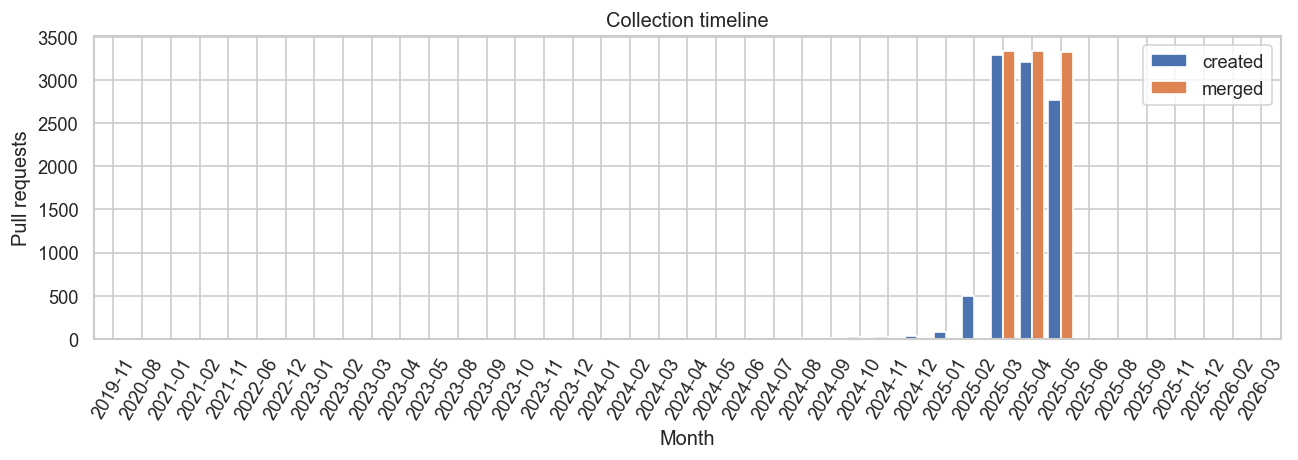
\includegraphics[width=\linewidth]{figures/data_understanding/collection_timeline.png}
    \caption{Pull request creation and merge month distribution.}
\end{figure}

The second question is whether the enriched fields are sufficiently complete. Pull request objects are present in 100.00\% of records, file lists in 99.99\%, full diffs in 99.96\%, formal reviews in 99.91\%, review comments in 99.82\%, and pull request comments in 99.78\%. Source files appear in 83.61\% of records. This is enough for analysis, although records without source files or source patches must be marked as lower quality.

\begin{figure}[htbp]
    \centering
    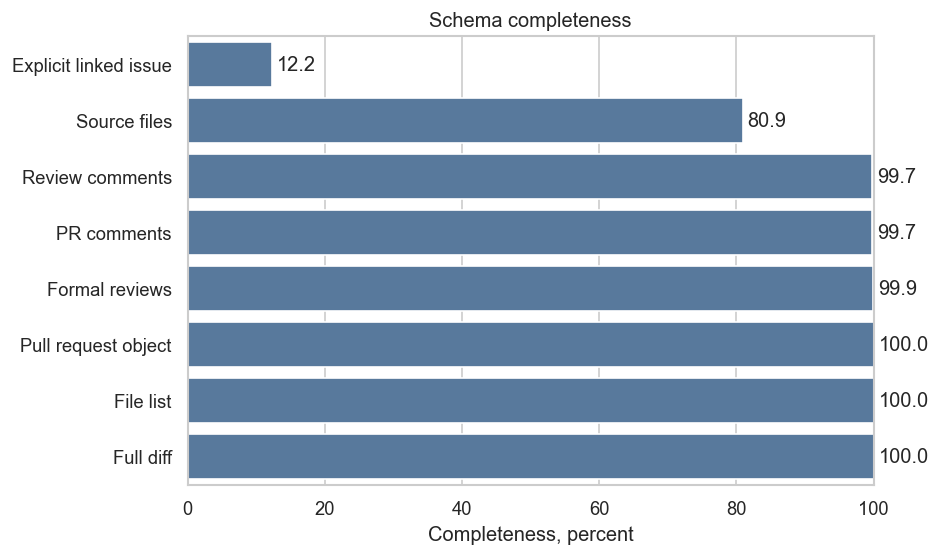
\includegraphics[width=\linewidth]{figures/data_understanding/schema_completeness.png}
    \caption{Completeness of key enriched fields.}
\end{figure}

The pull requests are mostly small to medium-sized, as intended by the candidate filter. The median pull request has 7 changed files and 261 changed lines. The distributions remain skewed, especially for additions, deletions, commits, and full-diff character count; therefore, the preparation stage uses capped tokenized diff embeddings instead of feeding complete diffs directly into a model.

\begin{figure}[htbp]
    \centering
    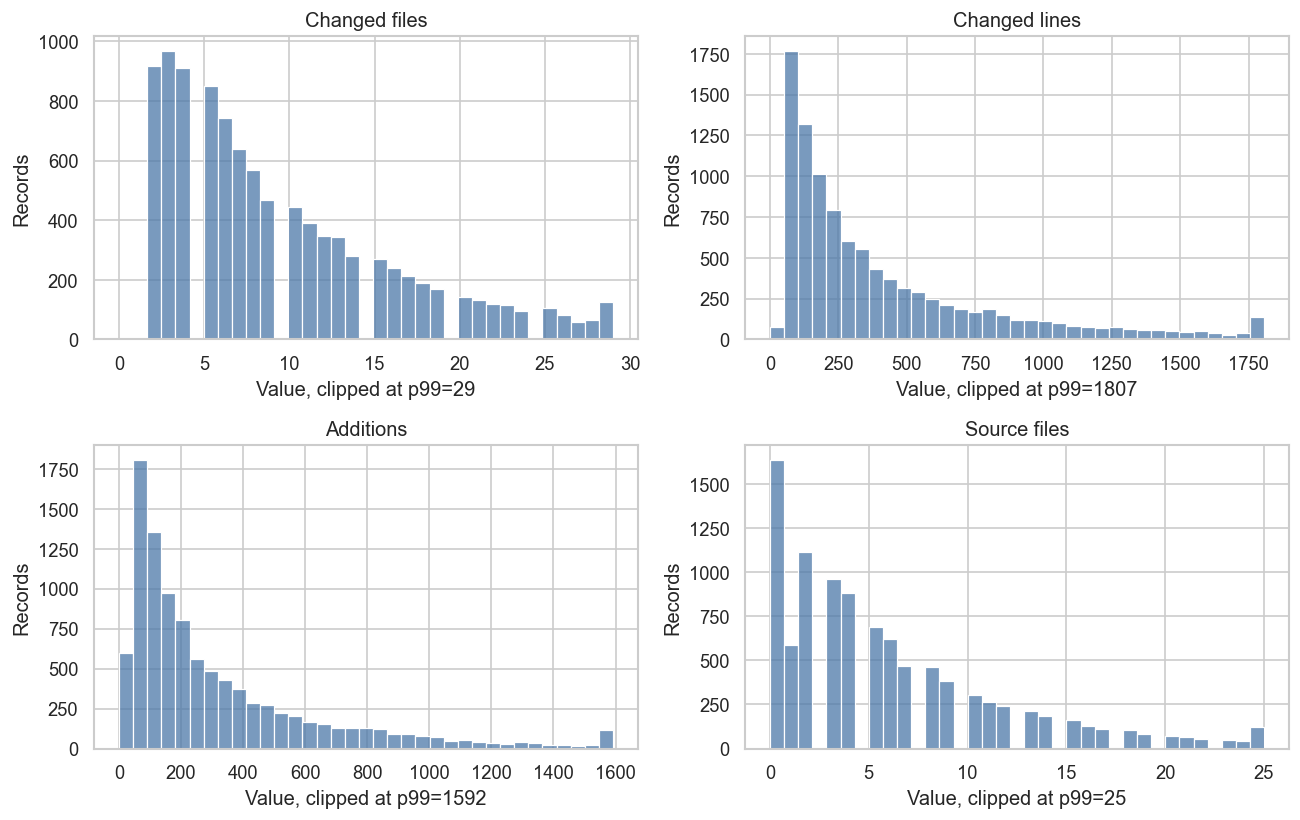
\includegraphics[width=\linewidth]{figures/data_understanding/size_distributions.png}
    \caption{Pull request size distributions.}
\end{figure}

Review activity is also skewed but sufficient. The median record has 6 formal reviews, 6 inline review comments, 6 meaningful review comments, and 3 pull request discussion comments. This supports the downstream target because most records contain enough reviewer activity to decide whether a concern was raised.

\begin{figure}[htbp]
    \centering
    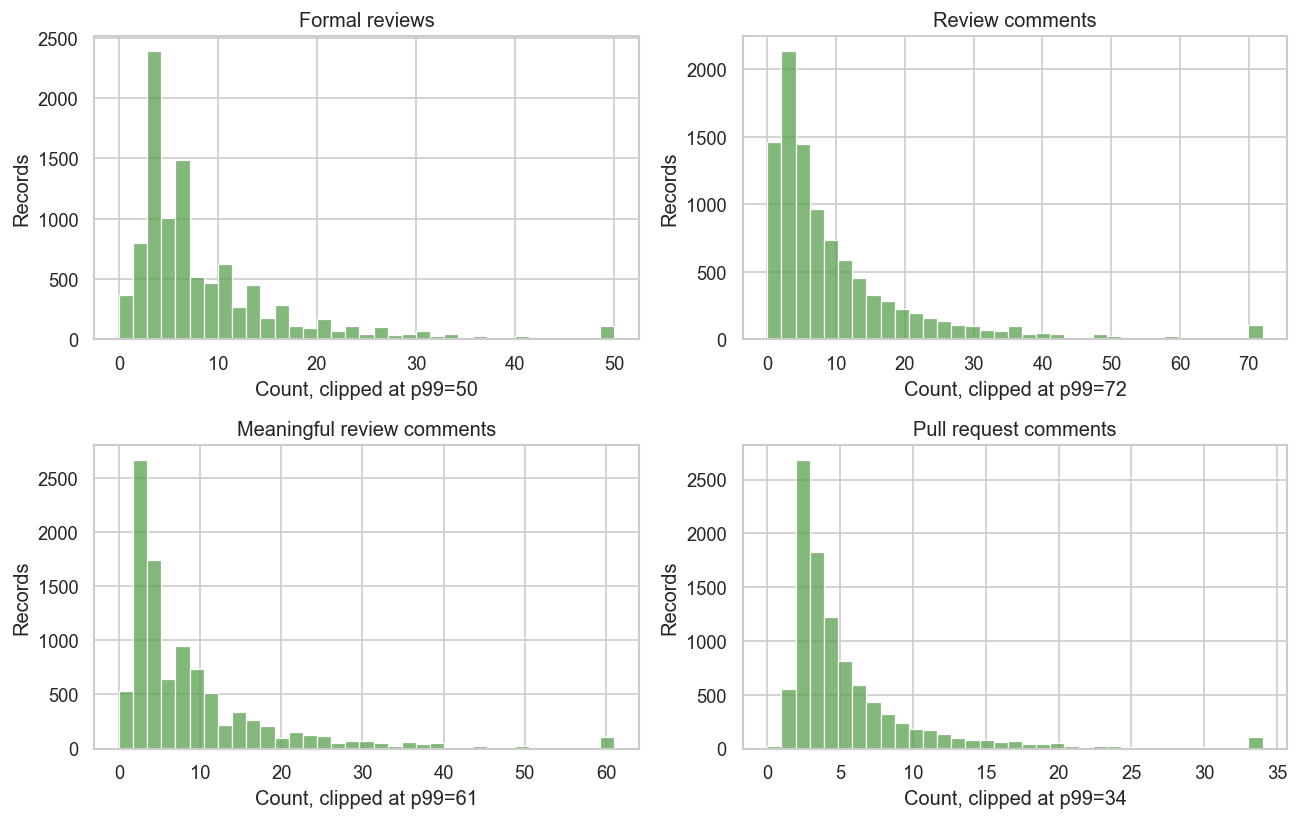
\includegraphics[width=\linewidth]{figures/data_understanding/review_activity.png}
    \caption{Review and discussion activity distributions.}
\end{figure}

The language distribution is diverse. TypeScript, Python, Java, Go, Rust, JavaScript, C++, C/C++, C\#, and Kotlin are the most common source languages. This is useful for the dataset goal because the model should not be tied to one ecosystem.

\begin{figure}[htbp]
    \centering
    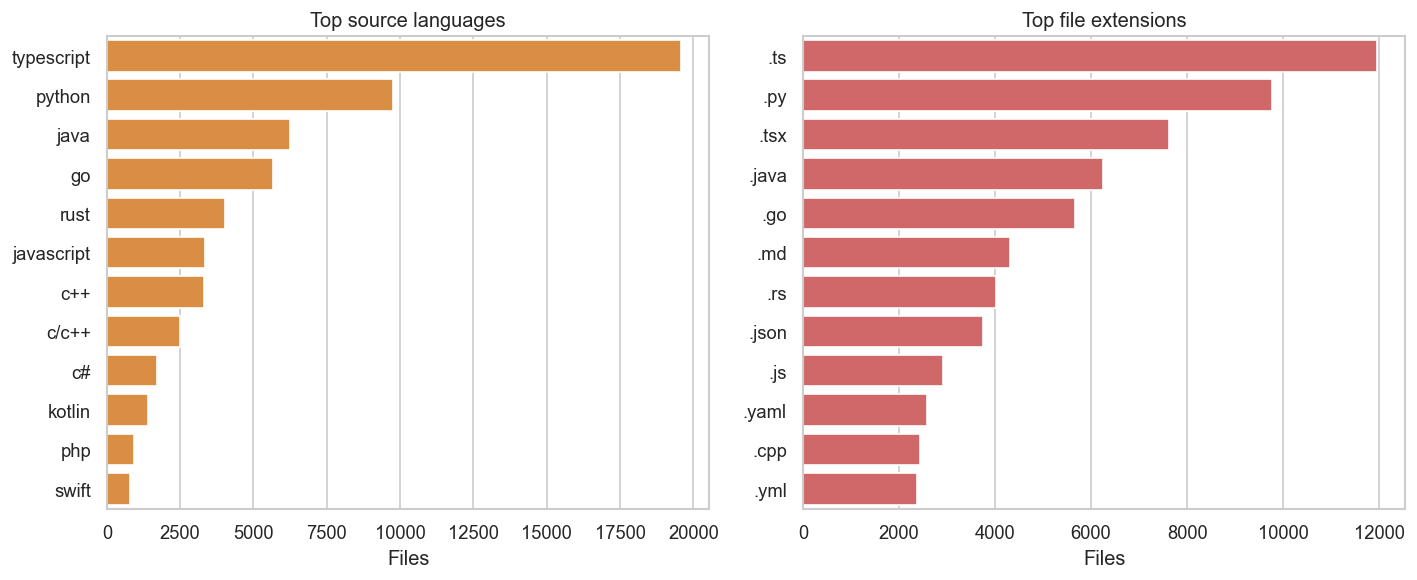
\includegraphics[width=\linewidth]{figures/data_understanding/language_distribution.png}
    \caption{Top source languages and file extensions.}
\end{figure}

Under the current quality filters, 7,373 records pass and 2,627 are rejected. The dominant rejection reasons are missing source-code patches, missing source files, insufficient discussion, insufficient meaningful review comments, and documentation-only changes. These failures are expected in public repository data and justify retaining quality metadata instead of assuming that every enriched pull request is modeling-ready.

\begin{figure}[htbp]
    \centering
    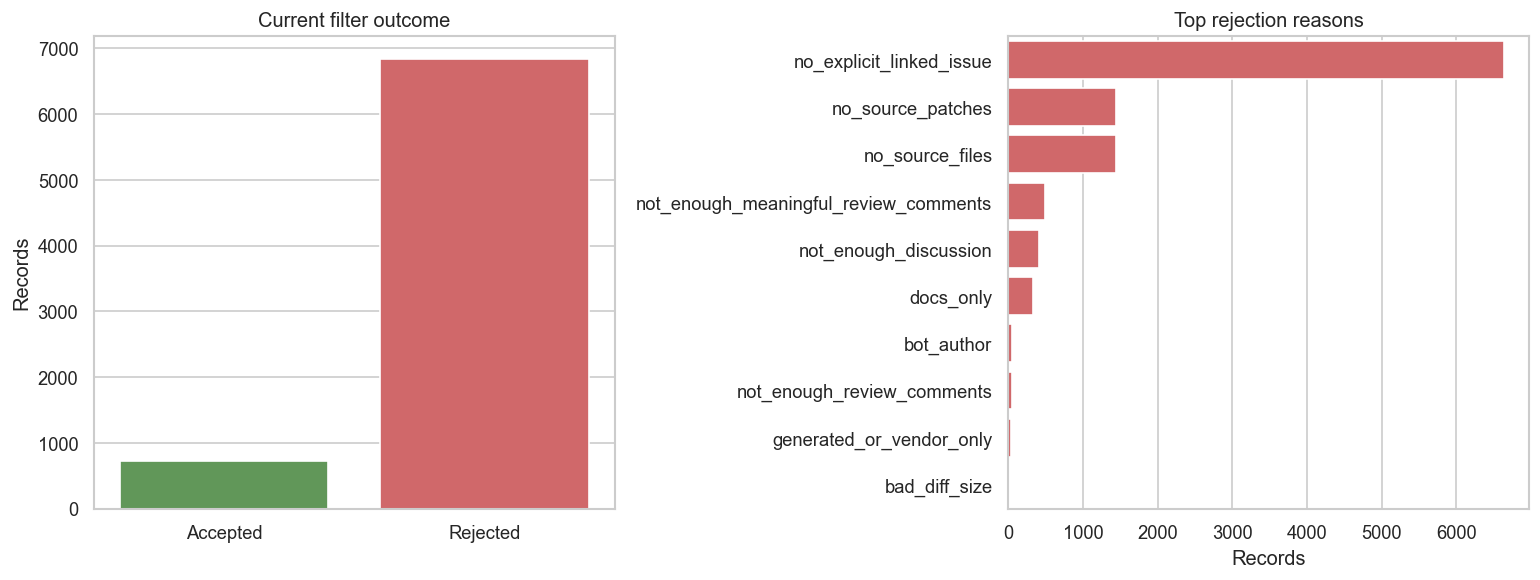
\includegraphics[width=\linewidth]{figures/data_understanding/quality_filters.png}
    \caption{Accepted versus rejected records and top rejection reasons under current filters.}
\end{figure}

\begin{figure}[htbp]
    \centering
    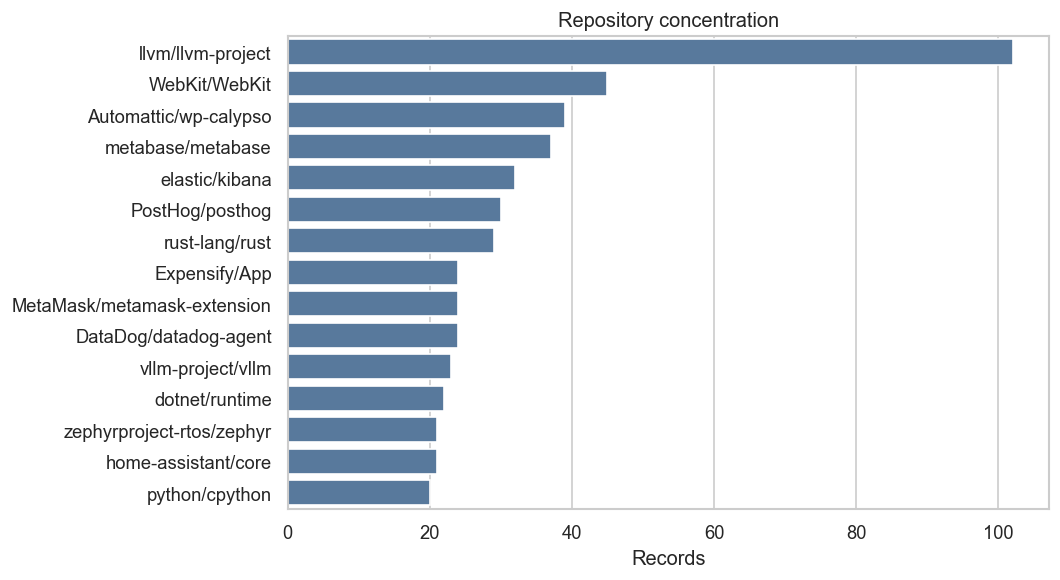
\includegraphics[width=\linewidth]{figures/data_understanding/repo_concentration.png}
    \caption{Top repositories by raw record count.}
\end{figure}

\subsection{Verify Data Quality}

The raw enrichment quality is sufficient for the next CRISP-DM stage. The dataset has enough scale, broad repository coverage, diverse languages, and high completeness for core pull request, review, comment, and diff fields. The main limitations are not missing metadata but unsuitable records: non-source changes, absent source patches, short discussions, and weak review-comment content.

Therefore, the raw file should not be used directly for modeling. It should first be transformed into a leakage-safe table, with quality flags retained for audit and with review-derived variables excluded from the feature matrix. The data is suitable for preparation and baseline modeling, with the later model interpreted as a proof of signal.
